
\documentclass[12pt]{article}
\usepackage[utf8]{inputenc}
\usepackage{graphicx}
\usepackage{amsmath}
\usepackage[margin=1in]{geometry}
\usepackage{indentfirst}
\usepackage{amsfonts}
\usepackage[portuguese]{babel}
\usepackage{float}
\usepackage[usenames,dvipsnames]{color}







\begin{document}

\begin{titlepage}

\newcommand{\HRule}{\rule{\linewidth}{0.5mm}} 
\center 
 

\textsc{\LARGE universidade de uoimbra}\\[1.5cm] % Name of your university/college
\textsc{\Large departamento de engenharia informática}\\[4cm] % Major heading such as course name
\textsc{\large compiladores}\\[1cm] % Minor heading such as course title


\HRule \\[0.5cm]
{ \huge \bfseries Compilador para a linguagem iJava}\\[0.4cm] 
\HRule \\[8cm]
 
\begin{minipage}{0.4\textwidth}
\begin{flushleft} \large
\emph{Autor:}\\
Bruno \textsc{Caceiro}  \\caceiro@student.dei.uc.pt
\end{flushleft}
\end{minipage}
~
\begin{minipage}{0.4\textwidth}
\begin{flushright} \large
\emph{Autor:} \\
David \textsc{Cardoso}  \\davidfpc@student.dei.uc.pt
\end{flushright}
\end{minipage}\\[2cm]



{\large \today}\\[3cm]

\vfill

\end{titlepage}



\section{Introdução}
Este projecto consiste no desenvolvimento de um compilador para a linguagem \emph{iJava} (imperative Java), que consiste num pequeno subconjunto da linguagem Java (versão 5.0). Os programas da linguagem \emph{iJava} são constituídos por uma única classe (a principal), contendo necessariamente um método \emph{main}, e podendo conter outros métodos e atributos, todos eles estáticos e (possivelmente) públicos.

O projecto foi estruturado em 3 fases, primeiramente foi feita a Análise Lexical, implementada na linguagem \emph{C} e utilizando a ferramenta \emph{lex}. A segunda fase consistiu na análise sintática, com a  construção da árvore de sintaxe abstrata e análise semântica (tabelas de símbolos, deteção de erros semânticos). No final foi feita a geração de código.

\begin{figure}[H]
       \centering
       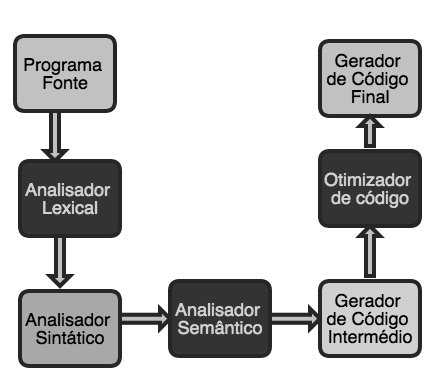
\includegraphics[keepaspectratio=true, width=300px]{fasesCompilacao.png}
       \caption{Fases de Compilação}
       \end{figure}


\section{Análise Lexical}

A Análise Lexical consiste em analisar a entrada de linhas de caracteres e produzir uma sequência de símbolos (\emph{tokens}) que podem ser manipulados mais facilmente por um \emph{parser}. É uma forma de verificar um determinado alfabeto, neste caso o alfabeto da linguagem \emph{iJava}.
Esta análise pode ser dividida em três fases:
\begin{itemize}
	\item Extração e classificação de \emph{tokens};
	\item Eliminação de delimitadores e comentários;
	\item Tratamento de erros;
\end{itemize}

O \emph{iJava} é um subconjunto da linguagem \emph{Java}, como tal, existe um conjunto de funcionalidades que embora não sejam suportadas, têm de ser consideradas. Assim, foi necessário tratar todo um conjunto de palavras reservadas de forma a permitir que sejam lexicalmente válidas mas não sintaticamente.
 


\section{Análise Sintática e Semântica}

\subsection{Árvore de Sintaxe Abstrata}

\subsection{Tratamento de Erros Lexicais}

\subsection{Análise Semântica}

\subsection{Tabela de Símbolos}

\subsection{Tratamento de Erros Semânticos}









	
	


\end{document}